\section{Mathematisches Modell der PMSM}\label{sec:math-pmsm}

Grundlegende Beschreibungen elektrischer Maschinen liefern Standardwerke, wie z.~B.\ \autocites{mullerII2008}{mullerI2005}{fischer2009}{schroder2000}.
In der vorliegenden Arbeit sind die in der Regel verwendeten linearisierten Spannungsgleichungen mit konstanten elektrischen Parametern allerdings nicht mehr ausreichend.
In dieser Arbeit werden Ansätze zur Erweiterung der linearisierten Gleichungen dargestellt.
Einige Ansätze unterteilen die absoluten Induktivitäten $L_d$ und $L_q$ in zwei Selbst- und Gegeninduktivitäten.
Bei \autocite{sturmberger} sind dabei sowohl die Selbst- als auch die Gegeninduktivität jeweils von de Strömen $i_d$ und $i_q$ abhängig.
In dieser Arbeit wird eine absolute Induktivität in $d-$ und $q-$Richtung verwendet.
Dies hat den Vorteil, dass bei Vereinfachungen wieder ein lineares Gleichungssystem entsteht.
Dabei werden allerdings die Eisenverluste nicht berücksichtigt.
Diese sind aber notwendig, um Induktivitäten zu messen und insbesondere den ohmschen Ständerwiderstand zu identifizieren \autocite{Kellner2012}.
Alle folgenden Anpassungen des Maschinenmodells beziehen sich weiterhin nur auf das Grundwellenverhalten der Maschine.
Eine Zusätzliche Betrachtung der Oberwelleneffekte wird innerhalb dieser Arbeit nicht weiter betrachtet.

Reduziert man die Synchronmaschine auf ihre grundlegenden elektrischen Eigenschaften so ergibt sich nach Abb.~\ref{fig:synchron-grundlage}: Drei Induktivitäten im Ständerblechpacket zusammen mit dem Permanentmagneten im Läufer.

\begin{figure}
\centering
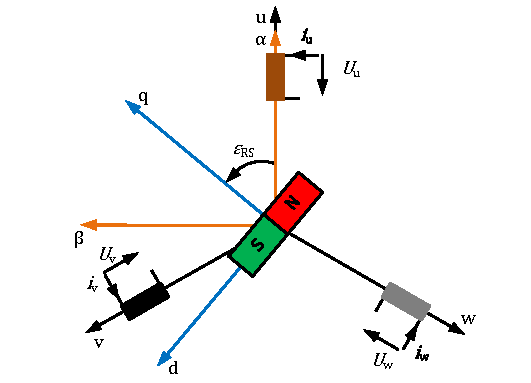
\includegraphics[width=\columnwidth]{img/synchron-grundlage}
\label{fig:synchron-grundlage}
\caption{Graphische Veranschaulichung der verschiedenen Koordinatensysteme, ständerfest $(\alpha, \beta)$ und rotorfest $(d, q)$.}
\end{figure}

Nach \textcite{ternesfeldkamp} und Transformation in das ständerfeste $(\alpha, \beta)$-Koordinatensystem ergibt sich die Spannungsleichung im rotorfesten System zu

\begin{align}
u_d &= R_1 i_d + \frac{d}{dt}\Psi_d - \omega_{el} \Psi_q \label{eqn:ud} \\ 
u_q &= R_1 i_q + \frac{d}{dt}\Psi_q + \omega_{el} \Psi_d \label{eqn:uq}
\end{align}

Allgemein lässt sich das daraus resultierende innere Drehmoment als

\begin{align}
M_i = \frac{3}{2} \underline{Psi}^{d,q} \times \underline{i}^{d,q} \label{drehmoment}
\end{align}

beschreiben.
Dabei wird vorausgesetzt, dass die Ständerwicklung symmetrisch und dreiphasig ist, der Strombelag nach \textcite{ternesfeldkamp} sinusförmig über dem Umfang verteilt und kein Nullsystem vorliegt.
Das innere Drehmoment $M_i$ für eine Maschine mit $p$ Polpaaren kann nach der Berechnung des Vektorproduktes als

\begin{align}
M_i = \frac{3p}{2}(\Psi_d i_q - \Psi_q i_d)
\end{align}

definiert werden.
Um das System vollständig zu beschreiben fehlt noch die Bewegungsgleichung nach \textcite{mullerI2005}.

\begin{align}
M_i - M_L = J \frac{d}{dt} \omega_{mech}
\end{align}

Bei diesem Modell sind alle Parameter konstant, die Ableitungen der Flussverkettungen, die in Gl.~\ref{eqn:ud} und Gl.~\ref{eqn:uq} verwendet werden unkompliziert zu bestimmen.
Aufgrund von Sättigungseffekten des Eisens sind insbesondere bei hochausgenutzten Maschinen die Induktivitäten der Synchronmaschine nicht mehr konstant, sondern vom Motorstrom abhängig \autocite{Kellner2012}.

\subsection{Linearisierte Gleichungen}\label{sec:lin-gleichungen}

Bei dem linearisierten Modell sind definitionsgemäß \autocite{mullerII2008} keine Sättigungserscheinungen vorhanden.
Alle elektrischen Parameter der Permanentmagneterregten Synchronmaschine und damit auch die Induktivitäten sind damit konstant.
Aus dieser Annahme folgt nach \textcite{ternesfeldkamp}, dass sich in läuferfesten $d, q-$Komponenten

\begin{align}
\Psi_d &= \Psi_pm + L_d i_d \\
\Psi_q &= L_q i_q
\end{align}

ergeben.
Die in $d-$Achse ausgerichteten Permanentmagnete rufen eine als konstant angenommene Flussverkettung $\Psi_pm$ hervor.
Daraus ergeben sich in Gl.~\ref{eqn:ud}, Gl.~\ref{eqn:uq} und Gl.~\ref{drehmoment} eingesetzt~--~die Grundgleichungen des linearen Maschinenmodells

\begin{align}
u_d &= R_1 i_d + L_d \frac{di_d}{dt} - \omega_{el}L_q i_q  \label{uq-allg} \\ 
u_q &= R_1 i_q + L_q \frac{di_q}{dt} + \omega_{el}L_d i_d + \omega_{el}\Psi_pm \label{ud-allg} \\ 
M_i &= \frac{3p}{2}(\Psi_pm i_q + (L_d - L_q)i_d i_q)
\end{align}

Die Spannungsgleichungen lassen sich gemäß Abb.~\ref{fig:spannungsgleichungen} graphisch darstellen.

\begin{figure}
\centering
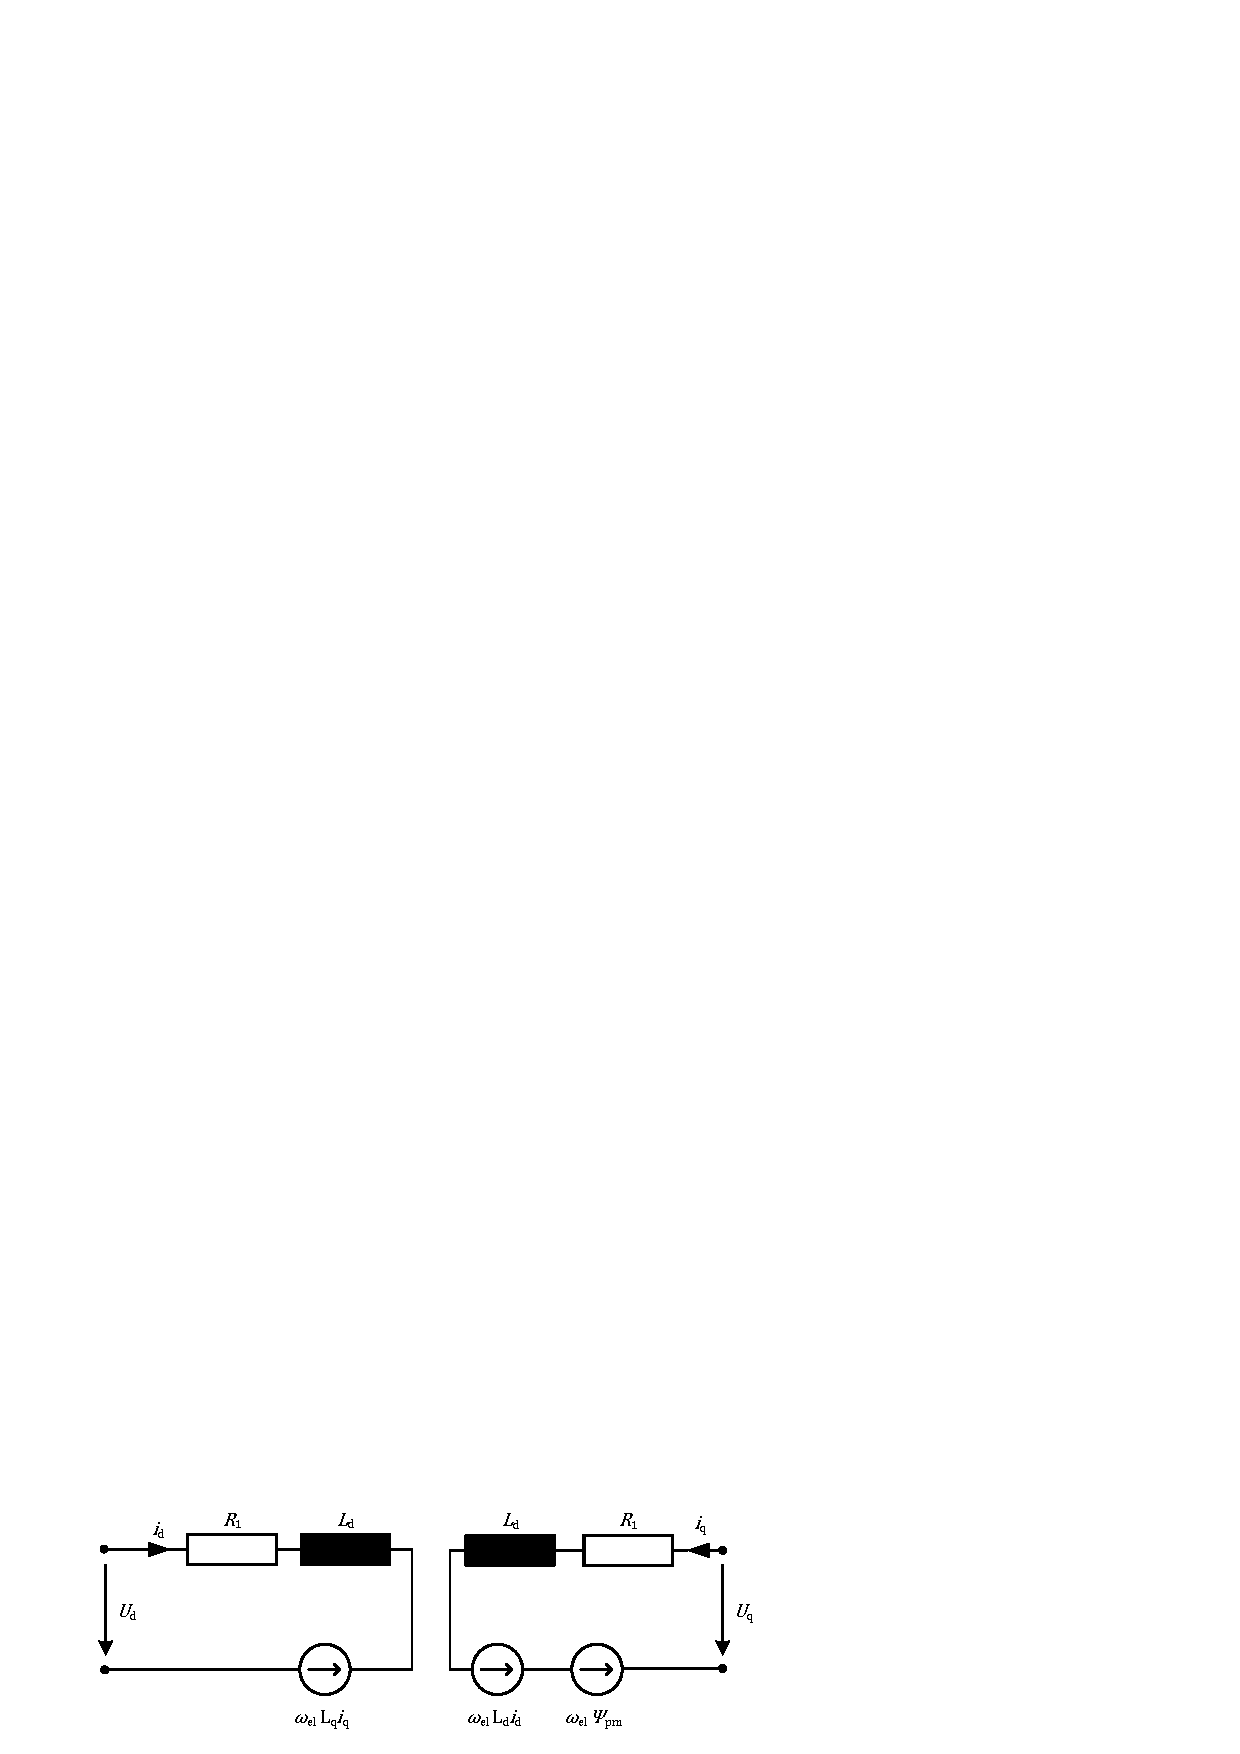
\includegraphics[width=\columnwidth]{img/spannungsgleichungen}
\label{fig:spannungsgleichungen}
\caption{Graphische Darstellung der Gleichungen \ref{ud-allg} und \ref{uq-allg}.}
\end{figure}
